

\section{Replication Results}

% latex table generated in R 3.3.1 by xtable 1.8-2 package
% Sun Aug 21 03:32:43 2016
\begin{table}[ht]
\centering
\begingroup\normalsize
\begin{tabular}{lccccc}
   & Logit & MRQAP & LSM & ERGM & AME \\ 
  \hline
\hline
Intercept/Edges & -4.44$^{\ast}$ & -4.24$^{\ast}$ & 0.94$^{\ast}$ & -12.17$^{\ast}$ & -3.39$^{\ast}$ \\ 
   & (0.34) &  & [0.09; 1.82] & (1.40) & [-4.38; -2.50] \\ 
  \textbf{Conflicting policy preferences} &  &  &  &  &  \\ 
  $\;\;\;\;$ Business vs. NGO & -0.86 & -0.87$^{\ast}$ & -1.37$^{\ast}$ & -1.11$^{\ast}$ & -1.37$^{\ast}$ \\ 
   & (0.46) &  & [-2.42; -0.41] & (0.51) & [-2.44; -0.47] \\ 
  $\;\;\;\;$ Opposition/alliance & 1.21$^{\ast}$ & 1.14$^{\ast}$ & 0.00 & 1.22$^{\ast}$ & 1.08$^{\ast}$ \\ 
   & (0.20) &  & [-0.40; 0.39] & (0.20) & [0.72; 1.47] \\ 
  $\;\;\;\;$ Preference dissimilarity & -0.07 & -0.60 & -1.76$^{\ast}$ & -0.44 & -0.79$^{\ast}$ \\ 
   & (0.37) &  & [-2.62; -0.90] & (0.39) & [-1.55; -0.08] \\ 
  \textbf{Transaction costs} &  &  &  &  &  \\ 
  $\;\;\;\;$ Joint forum participation & 0.88$^{\ast}$ & 0.75$^{\ast}$ & 1.51$^{\ast}$ & 0.90$^{\ast}$ & 0.92$^{\ast}$ \\ 
   & (0.27) &  & [0.86; 2.17] & (0.28) & [0.40; 1.47] \\ 
  \textbf{Influence} &  &  &  &  &  \\ 
  $\;\;\;\;$ Influence attribution & 1.20$^{\ast}$ & 1.29$^{\ast}$ & 0.08 & 1.00$^{\ast}$ & 1.09$^{\ast}$ \\ 
   & (0.22) &  & [-0.40; 0.55] & (0.21) & [0.69; 1.53] \\ 
  $\;\;\;\;$ Alter's influence indegree & 0.10$^{\ast}$ & 0.11$^{\ast}$ & 0.01 & 0.21$^{\ast}$ & 0.11$^{\ast}$ \\ 
   & (0.02) &  & [-0.03; 0.04] & (0.04) & [0.07; 0.15] \\ 
  $\;\;\;\;$ Influence absolute diff. & -0.03$^{\ast}$ & -0.06$^{\ast}$ & 0.04 & -0.05$^{\ast}$ & -0.07$^{\ast}$ \\ 
   & (0.02) &  & [-0.01; 0.09] & (0.01) & [-0.11; -0.03] \\ 
  $\;\;\;\;$ Alter = Government actor & 0.63$^{\ast}$ & 0.68 & -0.46 & 1.04$^{\ast}$ & 0.55 \\ 
   & (0.25) &  & [-1.08; 0.14] & (0.34) & [-0.07; 1.15] \\ 
  \textbf{Functional requirements} &  &  &  &  &  \\ 
  $\;\;\;\;$ Ego = Environmental NGO & 0.88$^{\ast}$ & 0.99 & -0.60 & 0.79$^{\ast}$ & 0.67 \\ 
   & (0.26) &  & [-1.32; 0.09] & (0.17) & [-0.38; 1.71] \\ 
  $\;\;\;\;$ Same actor type & 0.74$^{\ast}$ & 1.12$^{\ast}$ & 1.17$^{\ast}$ & 0.99$^{\ast}$ & 1.04$^{\ast}$ \\ 
   & (0.22) &  & [0.63; 1.71] & (0.23) & [0.63; 1.50] \\ 
  \textbf{Endogenous dependencies} &  &  &  &  &  \\ 
  $\;\;\;\;$ Mutuality & 1.22$^{\ast}$ & 1.00$^{\ast}$ &  & 0.81$^{\ast}$ & 0.39 \\ 
   & (0.21) &  &  & (0.25) & [-0.12; 0.96] \\ 
  $\;\;\;\;$ Outdegree popularity &  &  &  & 0.95$^{\ast}$ &  \\ 
   &  &  &  & (0.09) &  \\ 
  $\;\;\;\;$ Twopaths &  &  &  & -0.04$^{\ast}$ &  \\ 
   &  &  &  & (0.02) &  \\ 
  $\;\;\;\;$ GWIdegree (2.0) &  &  &  & 3.42$^{\ast}$ &  \\ 
   &  &  &  & (1.47) &  \\ 
  $\;\;\;\;$ GWESP (1.0) &  &  &  & 0.58$^{\ast}$ &  \\ 
   &  &  &  & (0.16) &  \\ 
  $\;\;\;\;$ GWOdegree (0.5) &  &  &  & 8.42$^{\ast}$ &  \\ 
   &  &  &  & (2.11) &  \\ 
   \hline
\hline
\end{tabular}
\endgroup
\caption{* p $<$ 0.05. Logistic regression and ERGM results are shown with standard errors in parentheses. MRQAP provides no standard errors. LSM and AME are shown with 95\% posterior credible intervals provided in brackets.} 
\label{tab:regTable}
\end{table}


\section{Capturing Network Stuff}

% \begin{figure}[ht]
% 	\centering
% 	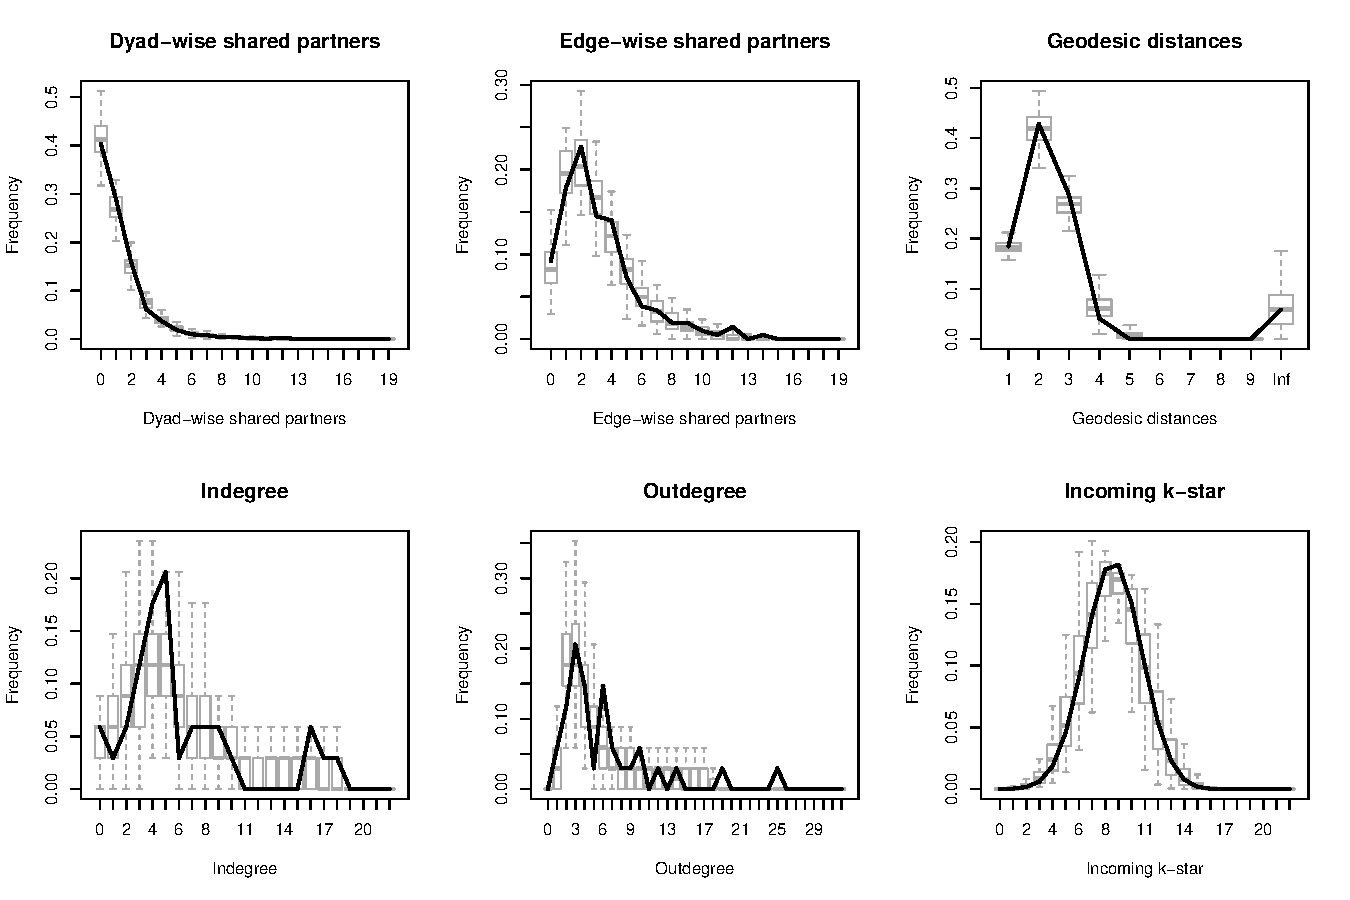
\includegraphics[width=.7\textwidth]{gof-ergm}
% 	\caption{ERGM network stuff}
% 	\label{fig:ergmNetGoF}
% \end{figure}

% \begin{figure}[ht]
% 	\centering
% 	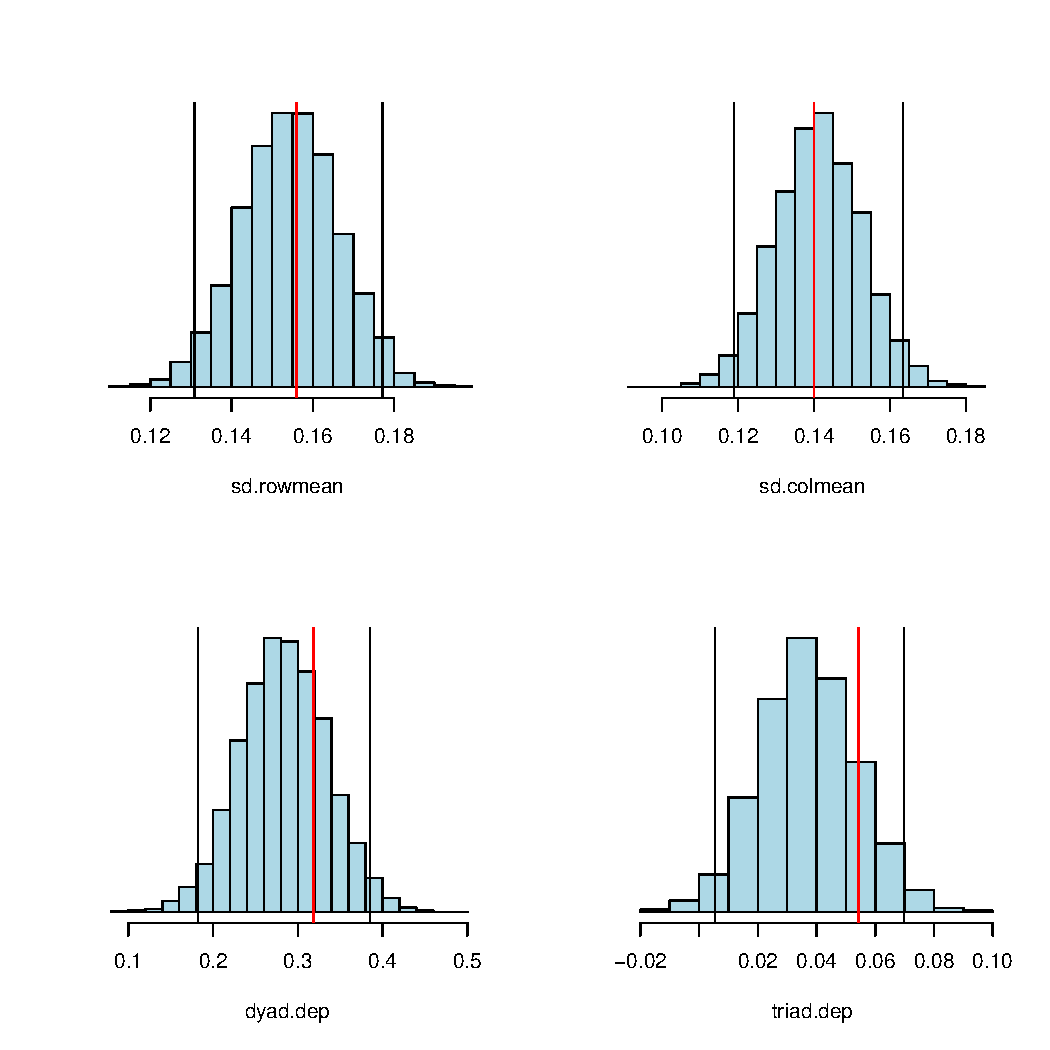
\includegraphics[width=.7\textwidth]{amenNetGoF}
% 	\caption{AMEN network stuff}
% 	\label{fig:amenNetGoF}
% \end{figure}

\section{Tie Formation Prediction}

% latex table generated in R 3.3.1 by xtable 1.8-2 package
% Tue Oct 18 00:16:48 2016
\begin{table}[ht]
\centering
\begingroup\normalsize
\begin{tabular}{lcc}
  & AUC & AUC (PR) \\ 
  \hline
\hline
AME & 0.99 & 0.94 \\ 
  LSM & 0.92 & 0.68 \\ 
  ERGM & 0.91 & 0.70 \\ 
  MRQAP & 0.88 & 0.67 \\ 
  Logit & 0.88 & 0.67 \\ 
  \end{tabular}
\endgroup
\caption{Area under the curve (AUC) comparison.} 
\label{tab:aucTable}
\end{table}


\begin{figure}[ht]
	\centering
	\begin{tabular}{cc}
	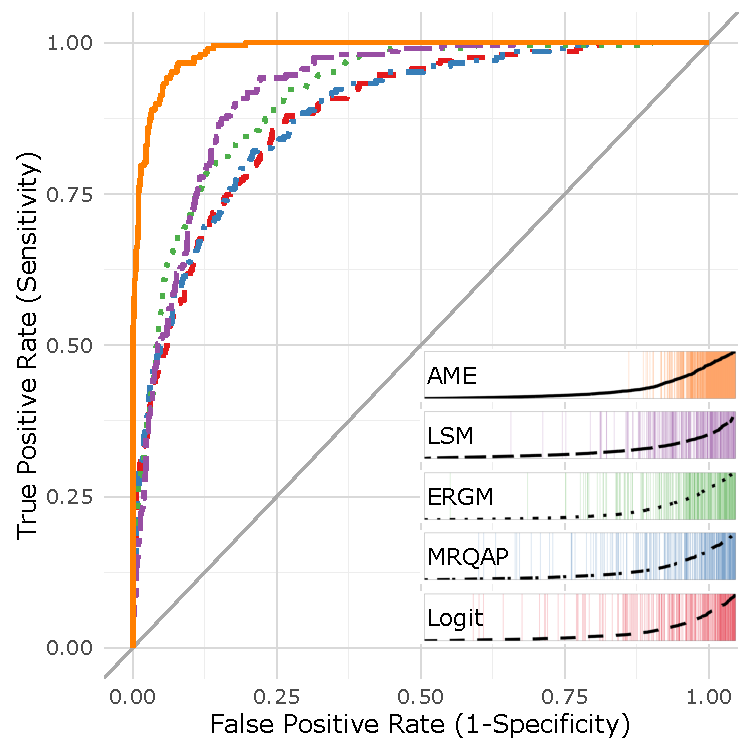
\includegraphics[width=.5\textwidth]{roc} & 
	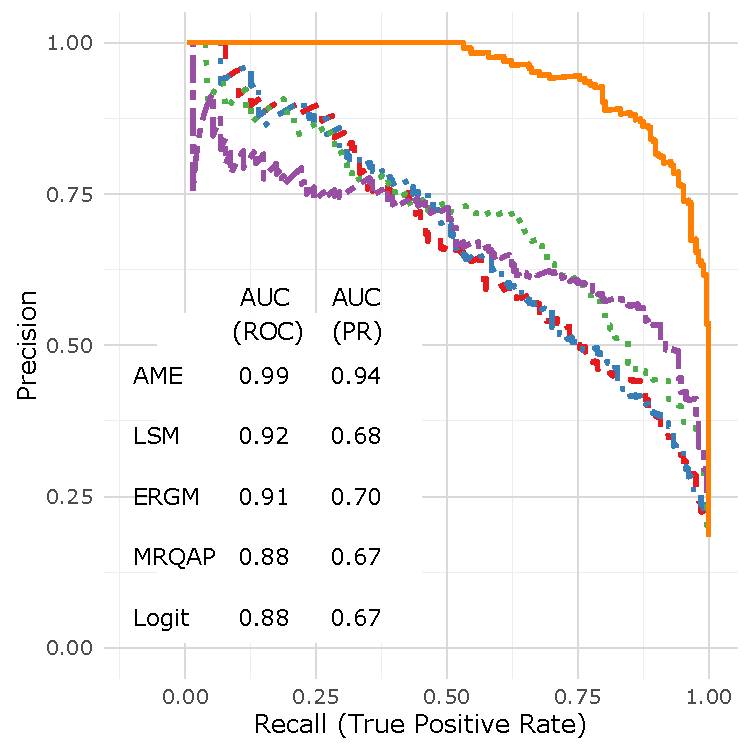
\includegraphics[width=.5\textwidth]{rocPr}	
	\end{tabular}
	\caption{ROC and separation plots}
	\label{fig:roc}
\end{figure}


\section{Latent Space Model Comparison}
% just in here for now for me to see what's going on with these models

% latex table generated in R 3.3.1 by xtable 1.8-2 package
% Sun Aug 21 03:38:39 2016
\begin{table}[ht]
\centering
\begingroup\tiny
\begin{tabular}{lccccc}
   & LSM & LSM (Bilinear) & LSM (SR) & LSM (Bilinear + SR) & AME \\ 
  \hline
\hline
Intercept/Edges & 0.94$^{\ast}$ & -2.66$^{\ast}$ & 0.60 & -2.50$^{\ast}$ & -3.39$^{\ast}$ \\ 
   & [0.09; 1.82] & [-3.53; -1.87] & [-1.10; 2.37] & [-4.14; -0.88] & [-4.38; -2.50] \\ 
  \textbf{Conflicting policy preferences} &  &  &  &  &  \\ 
  $\;\;\;\;$ Business vs. NGO & -1.37$^{\ast}$ & -2.64$^{\ast}$ & -3.07$^{\ast}$ & -2.87$^{\ast}$ & -1.37$^{\ast}$ \\ 
   & [-2.42; -0.41] & [-4.61; -0.96] & [-4.77; -1.56] & [-4.63; -1.29] & [-2.44; -0.47] \\ 
  $\;\;\;\;$ Opposition/alliance & 0.00 & 0.04 & 0.31 & 0.24 & 1.08$^{\ast}$ \\ 
   & [-0.40; 0.39] & [-0.44; 0.54] & [-0.24; 0.86] & [-0.36; 0.82] & [0.72; 1.47] \\ 
  $\;\;\;\;$ Preference dissimilarity & -1.76$^{\ast}$ & -2.00$^{\ast}$ & -1.88$^{\ast}$ & -2.20$^{\ast}$ & -0.79$^{\ast}$ \\ 
   & [-2.62; -0.90] & [-3.01; -1.03] & [-3.07; -0.68] & [-3.46; -0.96] & [-1.55; -0.08] \\ 
  \textbf{Transaction costs} &  &  &  &  &  \\ 
  $\;\;\;\;$ Joint forum participation & 1.51$^{\ast}$ & 1.24$^{\ast}$ & 1.56$^{\ast}$ & 1.62$^{\ast}$ & 0.92$^{\ast}$ \\ 
   & [0.86; 2.17] & [0.53; 1.93] & [0.69; 2.41] & [0.70; 2.52] & [0.40; 1.47] \\ 
  \textbf{Influence} &  &  &  &  &  \\ 
  $\;\;\;\;$ Influence attribution & 0.08 & -0.08 & 0.30 & 0.28 & 1.09$^{\ast}$ \\ 
   & [-0.40; 0.55] & [-0.62; 0.46] & [-0.37; 0.96] & [-0.42; 0.97] & [0.69; 1.53] \\ 
  $\;\;\;\;$ Alter's influence indegree & 0.01 & -0.05$^{\ast}$ & 0.06 & 0.05 & 0.11$^{\ast}$ \\ 
   & [-0.03; 0.04] & [-0.09; -0.01] & [-0.03; 0.14] & [-0.04; 0.13] & [0.07; 0.15] \\ 
  $\;\;\;\;$ Influence absolute diff. & 0.04 & 0.02 & -0.08$^{\ast}$ & -0.08$^{\ast}$ & -0.07$^{\ast}$ \\ 
   & [-0.01; 0.09] & [-0.03; 0.07] & [-0.14; -0.02] & [-0.14; -0.02] & [-0.11; -0.03] \\ 
  $\;\;\;\;$ Alter = Government actor & -0.46 & -0.80 & -0.11 & -0.20 & 0.55 \\ 
   & [-1.08; 0.14] & [-1.67; 0.04] & [-1.91; 1.76] & [-2.14; 1.74] & [-0.07; 1.15] \\ 
  \textbf{Functional requirements} &  &  &  &  &  \\ 
  $\;\;\;\;$ Ego = Environmental NGO & -0.60 & -1.90$^{\ast}$ & -1.69 & -1.84 & 0.67 \\ 
   & [-1.32; 0.09] & [-3.10; -0.86] & [-3.74; 0.23] & [-4.02; 0.11] & [-0.38; 1.71] \\ 
  $\;\;\;\;$ Same actor type & 1.17$^{\ast}$ & 1.40$^{\ast}$ & 1.82$^{\ast}$ & 1.90$^{\ast}$ & 1.04$^{\ast}$ \\ 
   & [0.63; 1.71] & [0.85; 1.95] & [1.10; 2.54] & [1.19; 2.62] & [0.63; 1.50] \\ 
   \hline
\hline
\end{tabular}
\endgroup
\caption{* p $<$ 0.05. 95\% posterior credible intervals are provided in brackets.} 
\label{tab:regTable_latSpace}
\end{table}


\begin{figure}[ht]
	\centering
	\begin{tabular}{cc}
	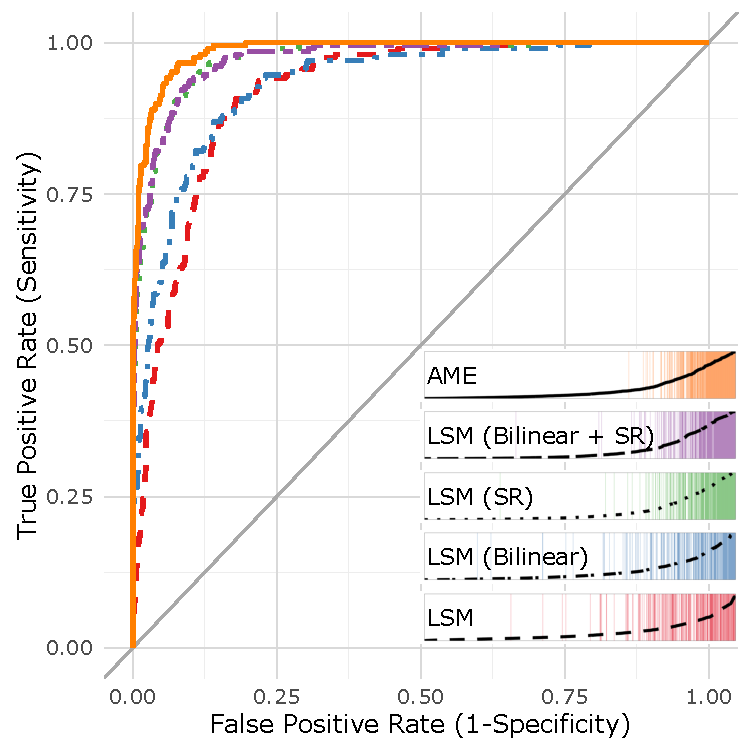
\includegraphics[width=.5\textwidth]{roc_latSpace} & 
	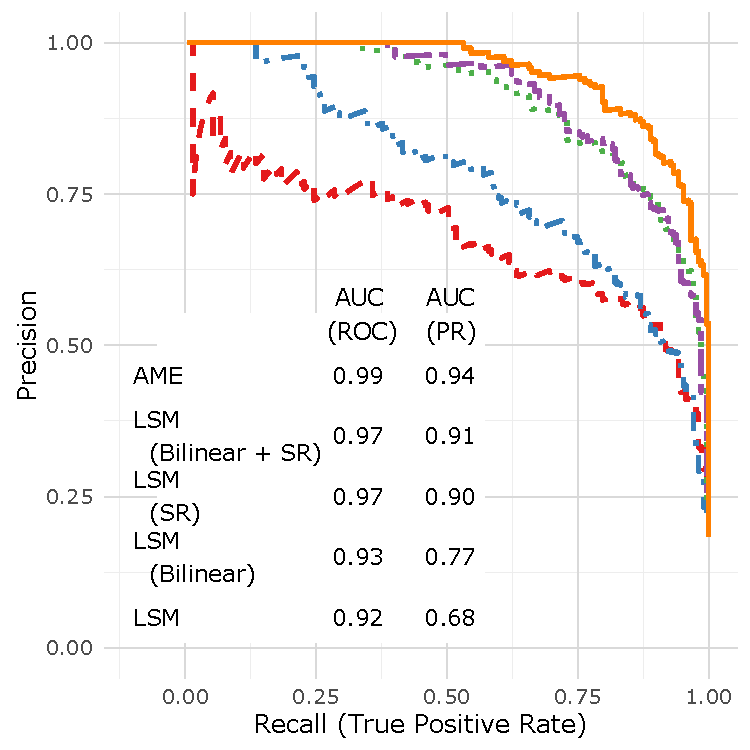
\includegraphics[width=.5\textwidth]{rocPr_latSpace}
	\end{tabular}
	\caption{ROC and separation plots}
	\label{fig:roc_latentSpace}
\end{figure}

\section{Conclusion}


\newpage
\section{Appendix}

\begin{figure}[ht]
	\centering
	\begin{tabular}{cc}
	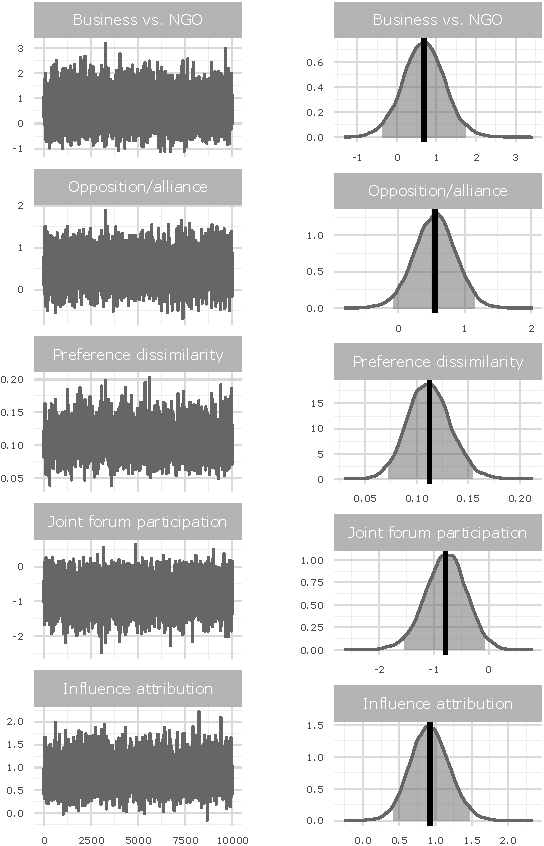
\includegraphics[width=.45\textwidth]{ameConv1} &
	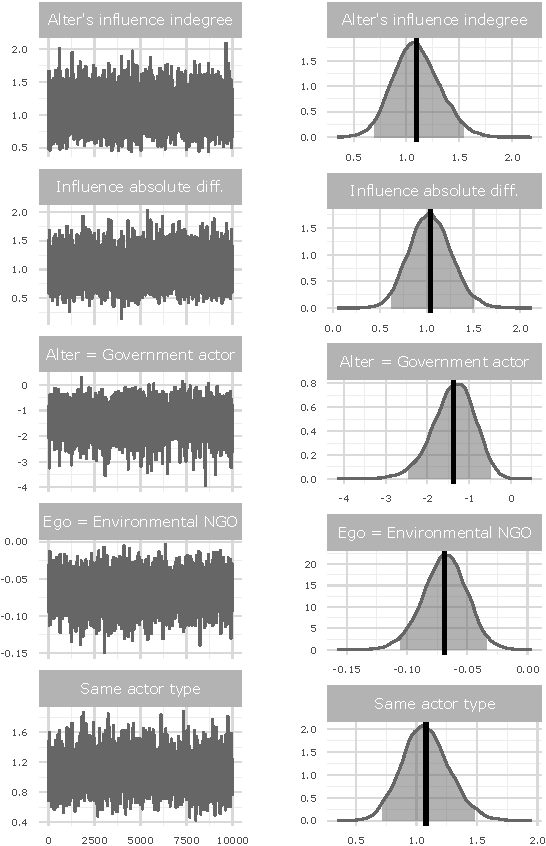
\includegraphics[width=.45\textwidth]{ameConv2}
	\end{tabular}
	\caption{ame convergence}
	\label{fig:ameConv}
\end{figure}

% FLoat code:

% \begin{figure}[ht]
% 	\centering
% 	\caption{Reciprocity coefficient estimates from each of the six-folds of the cross validation procedure.}
% 	\resizebox{1\textwidth}{!}{\input{../TeXoutput/crossvalCoef.tex}}
% 	\label{fig:crossval}
% \end{figure}

% \begin{figure}[ht]
%   \centering
%   \begin{tabular}{c}
% 	  \includegraphics[width=1\textwidth]{84net-crop} \\
% 	  \includegraphics[width=0.45\textwidth]{MapLegend}
%   \end{tabular}
%   \caption{Here we show the sanction network in 1984, nodes are colored by geographic coordinates of countries. Data for sanction cases comes from \citet{morgan2009threat}.}
%   \label{fig:spaghetti}
% \end{figure}
% \FloatBarrier

% \begin{figure}[ht]
% 	\centering
% 	\caption{Reciprocity plots}
% 	\begin{tabular}{ccc}

% 	\subfloat[sub1][Compliance: 1972]{
% 		\includegraphics[width=.5\textwidth]{compNet_1972}
% 		\label{fig:comp72}} & 

% 	\subfloat[sub1][Compliance: 1992]{
% 		\includegraphics[width=.5\textwidth]{compNet_1992}
% 		\label{fig:comp92}} \\

% 	\multicolumn{2}{c}{\subfloat[sub1][Compliance: 2012]{
% 			\includegraphics[width=.5\textwidth]{compNet_2012}
% 			\label{fig:comp02}}}


% 	\end{tabular}
% 	\label{fig:recipNet}
% \end{figure}

% \begin{table}[ht]
% 	\centering
% 	\begin{tabular}{lc}
% 		\hline\hline
% 		Outcome & Frequency \\
% 		\hline
% 		Capitulation by Sender After Imposition & 160 \\
% 		Stalemate after Sanctions Imposition & 71 \\
% 		\hline\hline
% 	\end{tabular}
% 	\caption{Outcomes of sanction cases no longer ongoing where compliance was not achieved.}
% 	\label{tab:termCases}	
% \end{table}